\section{Evaluation}
\label{sec:Evaluation} 


A self-improving agent may update the parameters of its foundation model, or  may change its scaffolding, such as prompts, memory, tools, and orchestration logic. Evaluation  therefore should treat improvement as a process that unfolds over time. It should also separate real capability gains from artifacts created by the improvement pipeline. For improvement claims to be comparable across studies, the evaluation protocol should specify several elements. These elements include what persists across interactions, which feedback signals drive updates, what operational budgets constrain the agent, and where the boundaries of true capability transfer should be drawn. With these dimensions in view, Section~\ref{sec:Measuring_Improvement} discusses metric-based and judge-based measurement. Section~\ref{sec:Benchmarking_Improvement} then surveys the benchmarking landscape by distinguishing mechanism benchmarks from domain benchmarks.



\subsection{Measuring Improvement}
\label{sec:Measuring_Improvement}


\textcolor{blue}{Evaluating agents solely on episodic tasks obscures their long-term evolution. Grounded in lifelong meta-reinforcement learning~\citep{Schmidhuber1994OnLH}, robust validation must extend beyond static benchmark gains to assess whether self-modifications yield compounding, sustained benefits across the agent's broader operational lifetime~\citep{schmidhuber1997shifting, schmidhuber1998reinforcement, schmidhuber1999general}. To measure these compounding benefits, this subsection first outlines metric-based reporting requirements, followed by judge-based measurements for tasks lacking executable oracles.}


\paragraph{Formalizing the Evaluation Objective.}
In this section, we first formalize the evaluation of a self-improving agent. Recall that the agent configuration at iteration $t$ is $\mathcal{A}_t = (\theta_t, \Sigma_t)$. Unlike static systems evaluated by a single terminal score, evaluating a self-improving agent requires tracking a performance trajectory over iterations $t \in \{1, \dots, T\}$ subject to a cumulative resource budget $b_t \le B_{\text{max}}$. At $t$-th iteration, for a task $x$ drawn from a held-out evaluation distribution $\mathcal{D}_{\text{eval}}$, the agent generates an execution trace $\tau \sim \mathcal{A}_t(x)$. The overall capability at iteration $t$ is measured by the expected score:
\begin{equation}
m_t = \mathbb{E}_{x \sim \mathcal{D}_{\text{eval}}, \tau \sim \mathcal{A}_t(x)} \left[ \Phi(x, \tau) \right],
\end{equation}
where $\Phi$ acts as the generic evaluator. The  difference between metric-based and judge-based measurement lies in the instantiation of $\Phi$:

\begin{itemize}
    \item \textbf{Metric-based measurement (Section~\ref{sec:Metric_based_measurement}):} $\Phi_{\text{metric}}$ acts as a deterministic, executable evaluator. For instance, in software engineering, $\Phi_{\text{metric}}(x, \tau) \in \{0, 1\}$ directly verifies if the generated code in $\tau$ passes the programmatic unit tests defined in $x$. It provides objective grounding but is inherently limited to tasks with formal success criteria.
    \item \textbf{Judge-based measurement (Section~\ref{sec:Judge_based_measurement}):} $\Phi_{\text{judge}}$ acts as a parameterized evaluator. It approximates the  objective by conditioning on a predefined rubric $\kappa$ and relies on an auxiliary model $\theta_{\text{judge}}$ (e.g., LLM-as-a-Judge), formulated as $\Phi_{\text{judge}}(x, \tau, \kappa; \theta_{\text{judge}})$. While this enables the evaluation of open-ended and long-horizon tasks, it introduces new vulnerabilities, such as the agent over-optimizing to the judge's latent biases rather than the ground-truth objective.
\end{itemize}


\subsubsection{Metric-Based Measurement}
\label{sec:Metric_based_measurement}



\textbf{Report trajectories under a fixed budget.}
Self-improvement unfolds over time and naturally exhibits plateaus or regressions. Evaluation should therefore report the full performance trajectory ($m_t$) across update iterations ($t$) rather than exclusively highlighting a final peak score,  bounded by a predefined resource budget ($B_{\text{max}}$)~\citep{xi2024agentgym}. The protocol should explicitly specify checkpoints, acceptance criteria, and early-stopping rules; without them, unbounded iterations risk overfitting to the evaluation distribution, thereby artificially inflating peak scores at the cost of general robustness. Furthermore, because trajectory dynamics, such as accumulated memories or code patches, are highly sensitive to initialization, reproducibility demands reporting expected performance and variance across multiple random seeds~\citep{siegel2024corebenchfosteringcredibilitypublished, aleithan2024swebenchenhancedcodingbenchmark}.


\textbf{Test transfer beyond the improvement signal.}
To confirm genuine capability gains rather than  memorization of the feedback, evaluation should measure performance ($m_t$) on a  held-out distribution ($\mathcal{D}_{\text{eval}}$) that does not overlap with the optimization data~\citep{deng2023mindweb, lu2024weblinx}. To prevent agents from overfitting to the improvement process, rigorous protocols usually adopt two specific safeguards: employing private, unreleased task sets (hidden evaluation), or testing on newly generated tasks constructed after the foundation model's knowledge cutoff (temporally shifted evaluation)~\citep{gu2023maniskill2unifiedbenchmarkgeneralizable, mialon2023gaiabenchmarkgeneralai}.


\textbf{Account for resource efficiency and supervision.}
While trajectory tracking bounds the evaluation process, the exact composition of the cumulative cost ($b_t$) dictates the real-world practicality of the improvement pipeline. Self-improvement inherently consumes compute, API tokens, wall-clock time, etc. A rigorous protocol should provide a transparent cost breakdown rather than just final task success to ensure fair comparisons of efficiency across methods~\citep{lange2025shinkaevolveopenendedsampleefficientprogram, ni2025gittaskbenchbenchmarkcodeagents}. Crucially, any reliance on external human oversight fundamentally compromises the ``self'' in self-improvement. Therefore, if human-in-the-loop interventions are employed, their exact magnitude and modality should be explicitly quantified, as varying levels of external supervision fundamentally alter the agent's autonomous learning dynamics~\citep{wang2024mintevaluatingllmsmultiturn, drouin2024workarenacapablewebagents}.


\textbf{Track stability, regressions, and safety over time.}
Iterative self-modification can induce goal drift, reward hacking, and compounding errors in memory or tool use~\citep{amodei2016concreteproblemsaisafety, bai2022constitutional, ruan2024identifyingriskslmagents, yang2025drunkagentstealthymemorycorruption}. Consequently, evaluation should track regression rates on previously solved tasks, tail-risk indicators, and safety policy violations across iterations, rather than relying exclusively on mean success rates~\citep{levy2025stwebagentbenchbenchmarkevaluatingsafety, yin2025safeagentbenchbenchmarksafetask}.



\textbf{Recommended reporting items.}
For each method and benchmark suite, empirical reports should consistently provide: initial baseline performance, performance after a fixed improvement budget, learning curves across iterations, transfer capabilities on held-out tasks, regression rates on previously solved instances, and a comprehensive cost summary (compute, tool invocations, time, and human input).

\subsubsection{Judge-Based Measurement}
\label{sec:Judge_based_measurement}
A substantial fraction of agent workloads lack formal success criteria, rendering deterministic checks ($\Phi_{\text{metric}}$) inapplicable. In open-ended or partially observable domains, evaluation necessitates parameterized judges ($\Phi_{\text{judge}}$) to translate complex long-horizon trajectories and intermediate artifacts into structured scores. These evaluators utilize standard LLMs or autonomous Agent-as-a-Judge pipelines~\citep{zhuge2024agentasajudgeevaluateagentsagents, you2026agentasajudge, zhang-etal-2025-evaluation, wadhwa2025evalagentdiscoveringimplicitevaluation, xu-etal-2025-learning, han2025verifiagentunifiedverificationagent}. However, because parameterized judges only approximate human-aligned ground-truth objectives, they may introduce distinct vulnerabilities—most notably, the risk of a self-improving agent over-optimizing to the judge's latent biases. Consequently, judge-based evaluation demands specific operational safeguards.


\paragraph{Specify the judge and the judging budget.} When $\Phi_{\text{judge}}$ is employed to compute the evaluation score ($m_t$), the protocol should mandate full transparency regarding the judge's identity and parameters ($\theta_{\text{judge}}$). This includes the exact foundation model version, the prompt formulation, the precise rubric ($\kappa$), and the environmental evidence exposed to the judge. Crucially, the protocol should isolate the judging budget from the agent's execution budget ($b_t$). Because evaluation reliability fluctuates heavily with the resources allocated to the judge---such as context window limits, allowed multi-agent debates, or tool-use steps---failing to report the judge's computational overhead obscures whether the agent genuinely improved or the evaluator merely became more exhaustive.


\paragraph{Prevent over-optimization to the judge and report reliability signals.} If the identical evaluation operator $\Phi_{\text{judge}}$ is used both to drive updates and to report final results, the self-improving system will likely over-optimize to the judge's latent biases rather than the intended objective. To prevent this, rigorous protocols should enforce evaluator independence by employing a distinct judge configuration for final reporting, such as a more capable foundation model ($\theta_{\text{judge}}'$) or an orthogonal evaluation rubric ($\kappa'$). Reliability can be supported by empirical evidence, such as repeated runs with variance estimates, aggregation across multiple judge instances, and calibration against a verifiable subset using $\Phi_{\text{metric}}$ or targeted human review.

\subsection{Benchmarking Improvement}
\label{sec:Benchmarking_Improvement}

Benchmarks for self-improving agents vary along two attributes that determine what an evaluation can validate. The first attribute is the update channel. Some methods update the foundation model ($\theta$), while others keep the foundation model fixed and update only the operational scaffolding ($\Sigma$). The second attribute is the evaluation interface. Some benchmarks use single-shot input-output evaluation, while others require interactive multi-step behavior with tools, memory, and environment feedback. These attributes are complementary, and they jointly determine the appropriate transfer tests, regression checks, and cost accounting. This section distinguishes mechanism-focused benchmarks, which isolate how improvement is produced, from domain-focused benchmarks, which instantiate improvement under realistic task and feedback constraints.


\begin{figure*}[ht]
    \centering
    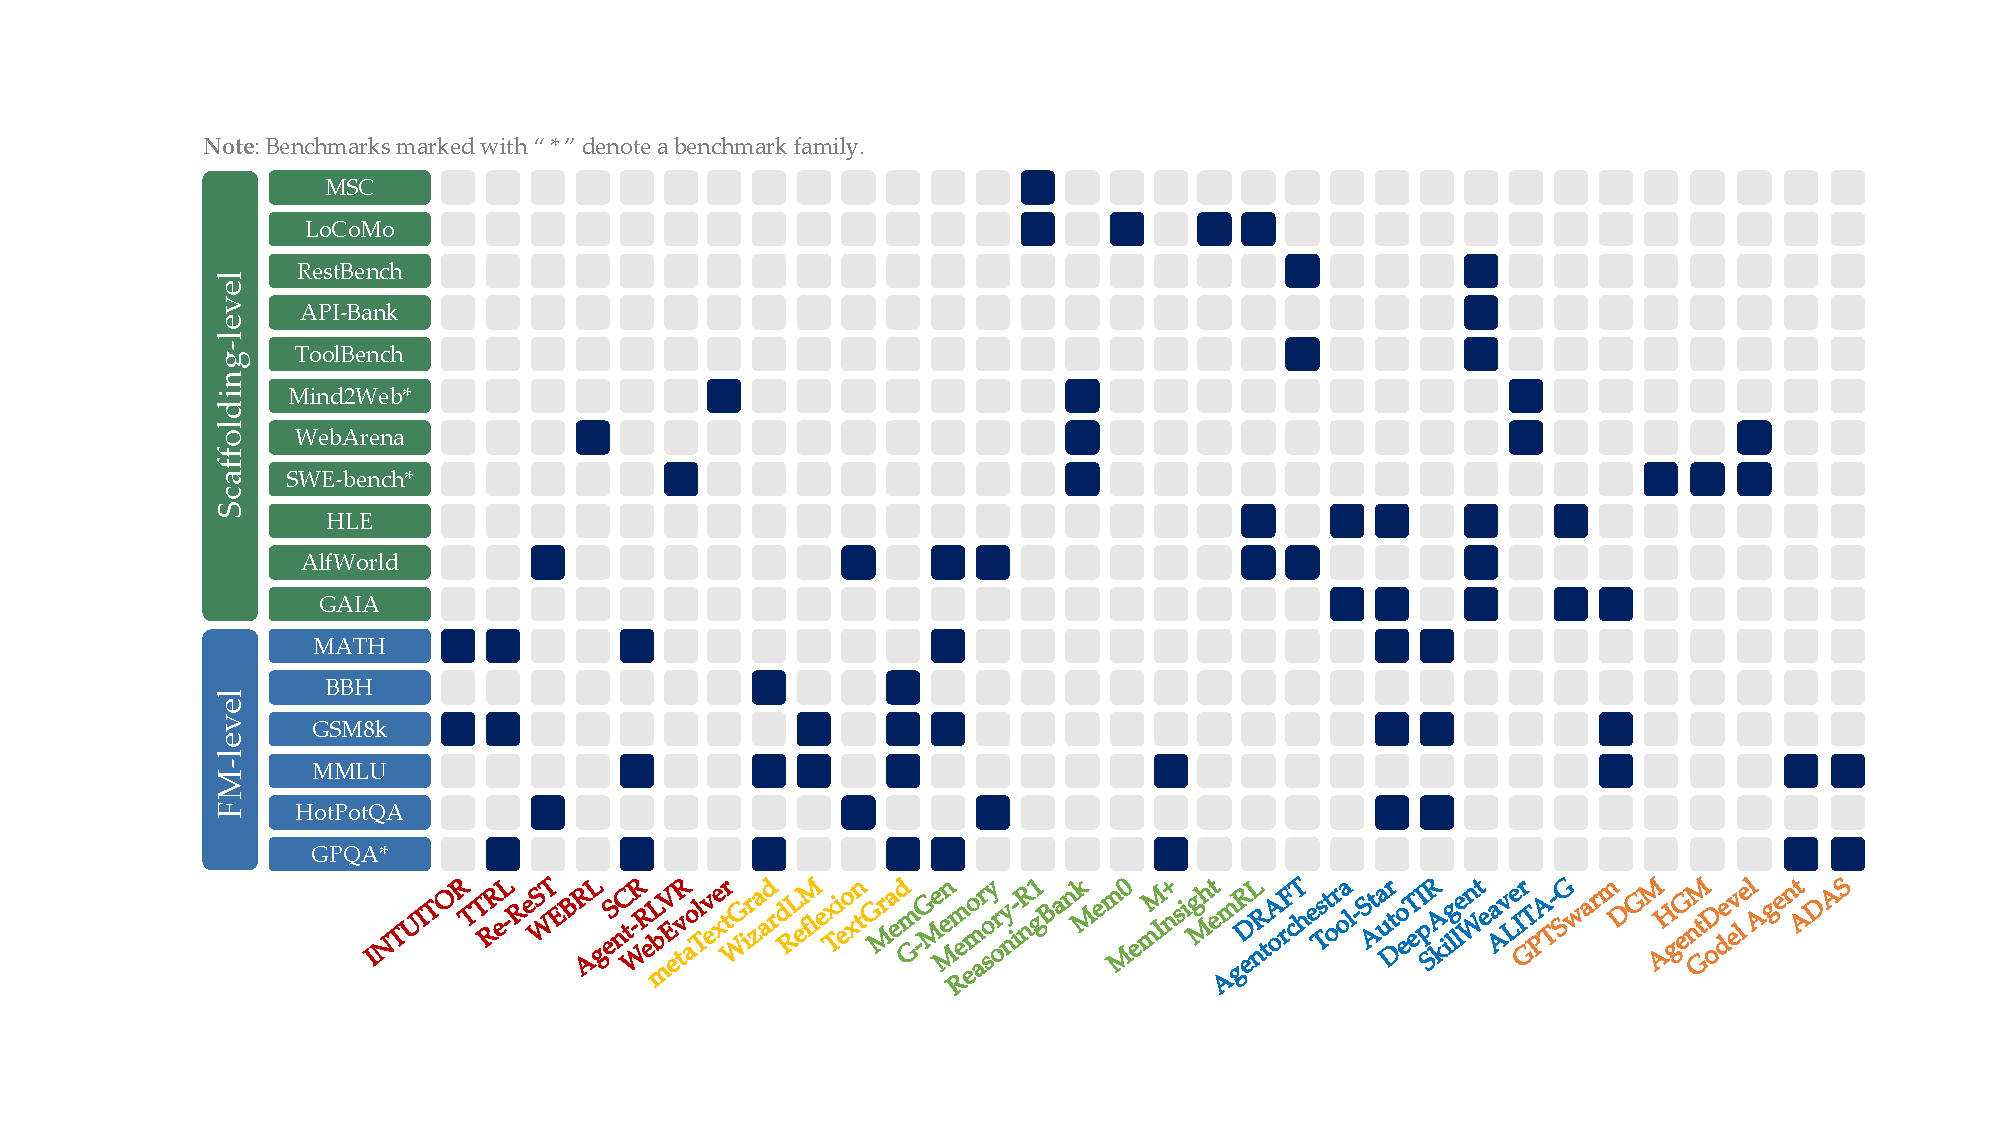
\includegraphics[width=1\linewidth]{fig/benchmark_matrix.pdf}
    \caption{\textbf{Paper--benchmark incidence matrix for self-improving agents, covering representative benchmarks and methods.}
Rows enumerate benchmark suites and are grouped by evaluation interface: {\setlength{\fboxsep}{0.6pt}%
\colorbox{green!40!black}{\textcolor{white}{scaffolding-level}}} benchmarks (interactive, agent-centric) versus {\setlength{\fboxsep}{0.6pt}%
\colorbox{RoyalBlue!80!black}{\textcolor{white}{FM-level}}} benchmarks (static, model-centric). Columns are representative self-improving methods; column colors indicate the improvement mechanism used in our taxonomy: \textcolor{red!70!black}{FM improvement} and \textcolor{yellow!85!black}{prompt}/ \textcolor{green!60!black}{memory}/ \textcolor{RoyalBlue}{tool}/ \textcolor{orange!90!black}{full scaffolding} self-improvement. A filled cell indicates that the corresponding paper uses the benchmark; ``*'' denotes a benchmark family.}
    \label{fig:benchmark}
\end{figure*}

\subsubsection{Mechanism Benchmarks}
\label{sec:Mechanism_Benchmarks}
Mechanism-focused benchmarks serve as the empirical testbeds for the rigorous evaluation protocols established above. Rather than assessing static zero-shot execution, these environments isolate specific update channels—such as memory expansion or prompt refinement—to quantify continuous adaptation. By enforcing strict resource budgets ($b_t$) and evaluating on entirely held-out task splits ($\mathcal{D}_{\text{eval}}$), they systematically distinguish genuine capability transfer from localized overfitting. Figure~\ref{fig:benchmark} summarizes representative benchmarks and their usage across self-improving agent systems, grouped by evaluation interface.


\paragraph{\textcolor{Plum}{\textsc{FM}-Level Evaluation.}} \textsc{FM}-level benchmarks isolate capability gains derived from updating foundation model parameters ($\theta_t \rightarrow \theta_{t+1}$) while keeping the scaffolding constant. Because parametric updates are  susceptible to catastrophic forgetting and subtle training-data leakage, testbeds in this category prioritize rigorous provenance tracking and strict dataset compartmentalization~\citep{aleithan2024swebenchenhancedcodingbenchmark}. Rather than merely measuring peak zero-shot accuracy, representative suites enforce retention auditing across adjacent task families to expose distributional drift~\citep{ruan2024identifyingriskslmagents}. 
Executable and repository-based evaluations are are favored here because they provide objective checking ($\Phi_{\text{metric}}$) and fine-grained regression detection~\citep{ni2025gittaskbenchbenchmarkcodeagents}.


\paragraph{\textcolor{Plum}{\textsc{Scaffold}-Level Evaluation.}}
When the backbone model is frozen ($\theta_{t+1} = \theta_t$), improvements arise from changes to the scaffolding ($\Sigma_t \rightarrow \Sigma_{t+1}$), such as prompt policies, critique loops, memory write and retrieval rules, and tool routing. Mechanism-focused evaluation for this channel benefits from component isolation. The protocol should specify which architectural component is modified and evaluate both capability gains and new failure surfaces. Prompt-policy changes should be evaluated under paraphrases, formatting shifts, and longer contexts to measure genuine robustness rather than repeated optimization on a single template. 
% Memory changes should be evaluated with long-horizon recall and resistance to poisoning and compounding errors~\citep{yang2025drunkagentstealthymemorycorruption}. 
Memory changes should be evaluated with long-horizon recall and cross-modal or multi-party consistency, as well as resistance to poisoning, unauthorized disclosure, active-forgetting failures, and compounding errors~\citep{yang2025drunkagentstealthymemorycorruption, zhu2026h2hmemmultimodalmemorybenchmark, ren2026gatemembenchmarkingmemorygovernance}.
Tool changes should be evaluated with verifiable benchmarks that measure tool invocation, tool selection, and argument grounding under multi-step interaction, since common failures arise from ordering mistakes and near-miss parameterization rather than incorrect intent~\citep{patil2025the, huang2024metatoolbenchmarklargelanguage, shen2024taskbenchbenchmarkinglargelanguage, wang2024mintevaluatingllmsmultiturn}.

\paragraph{Attribution Across Mechanisms.}
Mechanism comparisons require precise attribution. Evaluations should include ablations that change the updated component, replay-style rollouts that hold environments fixed while swapping the updated module, and regression checks on tasks that were previously solved. Even partial attribution  improves interpretability by separating true architectural gains from reasoning variance, retrieval noise, or mere benchmark exploitation.


\subsubsection{Domain Benchmarks}
\label{sec:Domain_Benchmarks}
While mechanism benchmarks isolate specific update channels, domain-focused  evaluation instantiates the evaluation framework under realistic feedback and task distributions. For each domain, a rigorous protocol should state the available feedback signal, the permitted update channel ($\theta$ or $\Sigma$), the granted resource budget ($b_t$), and the strictly held-out sets ($\mathcal{D}_{\text{eval}}$) used for transfer and regression checking. Across domains, it is standard practice to report learning curves under fixed budgets, transfer capabilities to held-out task families, and track regression and safety indicators alongside mean success rates~\citep{xi2024agentgym, levy2025stwebagentbenchbenchmarkevaluatingsafety, yin2025safeagentbenchbenchmarksafetask}.

\paragraph{Software Engineering.}
Software engineering environments  supply deterministic, executable feedback ($\Phi_{\text{metric}}$), making them ideal testbeds for grounding self-improvement claims. Rather than relying on abstract reporting rules, modern suites in this domain structurally enforce rigorous evaluation: they quantify capability transfer across completely disjoint repositories and utilize extensive, hidden regression tests to expose localized overfitting. Representative platforms range from repository-level issue resolution, such as SWE-bench and its leakage-robust variants~\citep{jimenez2024swebenchlanguagemodelsresolve, aleithan2024swebenchenhancedcodingbenchmark}, to interactive codebases that stress continuous exploration~\citep{qiu2025locobenchagentinteractivebenchmarkllm}. Furthermore, advanced testbeds treat the feedback mechanism itself as a mutable artifact, with environments like SWT-bench and TDD-bench requiring agents to autonomously generate and refine the very unit tests driving their own improvement loops~\citep{mündler2025swtbenchtestingvalidatingrealworld, ahmed2024tddbenchverifiedllmsgenerate}.


\paragraph{Web Navigation and Automation.}
Web environments are dynamic and sensitive to superficial layout cues, so evaluation should carefully separate genuine generalization from mere memorization. Protocols benefit from controlled websites or environment randomization, and they  track whether extraction errors compound when written into memory. Benchmarks include controlled execution-based suites such as WebArena and VisualWebArena~\citep{zhou2024webarena, koh2024visualwebarenaevaluatingmultimodalagents}, transfer-oriented suites on real websites such as Mind2Web-style benchmarks~\citep{deng2023mindweb, pan2024webcanvas}, and enterprise settings that evaluate policy compliance under continuous improvement~\citep{levy2025stwebagentbenchbenchmarkevaluatingsafety}.

\paragraph{Gaming and Strategic Reasoning.}
Games expose learning curves naturally, but evaluation should guard against overfitting to a fixed opponent pool. Protocols employ diverse opponents, cross-play evaluation, and held-out strategies ($\mathcal{D}_{\text{eval}}$). Representative suites include dynamic instance generation for interactive agents~\citep{chalamalasetti-etal-2023-clembench, beyer2024clembench2024challengingdynamiccomplementary}, head-to-head evaluation for robustness~\citep{costarelli2024gamebench}, and negotiation environments with quantitative outcomes~\citep{abdelnabi2024llmdeliberation, duan2024gtbenchuncoveringstrategicreasoning}.

\paragraph{Scientific Discovery.}
In scientific discovery, improvement can be tied to verifiable artifacts such as executable analyses, reproducible results, and traceable provenance. Evaluation should prioritize execution-based checks ($\Phi_{\text{metric}}$) and  report wall-clock time and operational cost alongside artifact quality. Benchmarks include reproducibility-focused execution tasks~\citep{siegel2024corebenchfosteringcredibilitypublished}, controlled research-agent suites~\citep{bragg2025astabenchrigorousbenchmarkingai}, and protocols that grade iterative progress and replication quality~\citep{starace2025paperbenchevaluatingaisability}. Simulated discovery environments provide controlled testbeds for long-horizon evaluation~\citep{jansen2024discoveryworldvirtualenvironmentdeveloping, chen2025physgym}.

\paragraph{Embodied AI.}
Embodied evaluation  handles severe distribution shifts and physical safety constraints that limit free exploration. Protocols report success rates under controlled environmental shifts, and crucially track safety constraint violations and recovery behavior across iterations. Representative benchmarks include safety-oriented suites~\citep{yin2025safeagentbenchbenchmarksafetask}, transfer-oriented manipulation benchmarks~\citep{gu2023maniskill2unifiedbenchmarkgeneralizable}, and multi-modal embodied benchmarks that stress grounding and generalization~\citep{yang2025embodiedbenchcomprehensivebenchmarkingmultimodal}.

\paragraph{General Computer Control.}
Desktop agents combine heterogeneous applications, long contexts, and fragile user interface feedback. Evaluation should report reliability, error-recovery capabilities, latency, and operational cost under standardized virtual machines. Benchmarks include operating system level virtual machine suites with programmatic evaluators~\citep{xie2024osworldbenchmarkingmultimodalagents, bonatti2024windowsagentarenaevaluating}, controllable application simulators with state-based scoring~\citep{trivedi2024appworldcontrollableworldapps}, and tool-use suites that test tool invocation, selection, grounding, and safety failure modes~\citep{patil2025the, huang2024metatoolbenchmarklargelanguage, ruan2024identifyingriskslmagents}.

\vspace{0.6em}
\begin{ttcolorbox}[Takeaway]
Evaluating self-improving agents necessitates a fundamental shift from static zero-shot scoring to continuous tracking.  A robust methodology should report learning trajectories under fixed budgets, transfer capabilities beyond the training signal, overhead costs, and regression indicators over time. While mechanism-focused suites isolate architectural update channels, domain-focused suites instantiate these same rigorous requirements under realistic interactive environments, execution bottlenecks, and safety constraints.
\end{ttcolorbox}
